\documentclass[12pt,a4paper,openright,twoside]{article}

\usepackage[italian]{babel}

\usepackage[utf8x]{inputenc}
\usepackage{caption}
\usepackage{geometry}
\usepackage{float}
\usepackage{wrapfig}
\usepackage{graphicx}
\usepackage{caption}
\usepackage{subcaption}
\usepackage{listings}
\usepackage{color}

\usepackage{mwe}
\usepackage{graphbox} %loads graphicx package


\usepackage{fancyhdr}


\usepackage{indentfirst}

\usepackage{graphicx}

\usepackage{newlfont}

\usepackage{amssymb}
\usepackage{amsmath}
\usepackage{latexsym}
\usepackage{amsthm}

\usepackage{mathtools}
\usepackage{pdfpages}

\usepackage{subfig}

\begin{document}

\section{Valutazione di sistemi esistenti}

In questa fase si sono analizzate applicazioni concorrenti già inseriti nei market più famosi di dispositivi mobili, per evidenziare problemi di usabilità (metriche quantitative e qualitative di usabilità utili come input per la fase di design e per un confronto successivo).\\
Individuata la categoria più adatta (\textit{Stile di vita} su \textit{Google Play Store} / \textit{Ristoranti e bar} su \textit{Microsoft Store}), abbiamo individuato due app strutturalmente
diverse, ma che a prima analisi sono dei buoni modelli di partenza al fine di progettare la nostra applicazione.\\
Abbiamo analizzato:
\begin{itemize}
\item \textbf{”Giallo Zafferano”}\\
Sviluppatore: Banzai Media\\
Installazioni: 1.000.000-5.000.000 su Google Play\\
Piattaforme compatibili: Android, iOS, Windows Phone/Store\\
Punteggio: 4,2/5 su 26.621 recensioni\\
Versione analizzata: app tablet Windows Store\\
Lingua: Italiano\\
\item \textbf{”Allthecooks”}\\
Sviluppatore: Allthecooks, LLC.\\
Installazioni: 10.000.000-50.000.000 su Google Play\\
Piattaforme compatibili: Android, iOS, Windows Phone/Store, Smartwatch\\
Punteggio: 4,3/5 su 46.678 recensioni\\
Versione analizzata: app tablet Windows Store\\
Lingua: Inglese\\
\end{itemize} 

\subsection{Expert Usability Review}
Procediamo ora con l'expert usability review, ovvero l'analisi dell'usabilità di un software o piattaforma web da parte di un esperto di usabilità. A tal proposito ci avvarremo del consulto di Alessandro D'Andrea, Business Analyst di Yoox.com, al fine di verificare pregi e difetti dell'usabilità riscontrati nelle due applicazioni.\\
L'analisi si divide in diverse fasi:
\begin{itemize}
\item Definizione delle linee guida adatte e prima dell'esplorazione
\item Analisi dell'architettura
\item Analisi diretta: sistema VS linee guida
\item Analisi inversa: linee guida VS sistema
\item Rilevazione di un numero ragionevole di errori
\item Identificazione dei task del sistema
\item Identificazione del target di utenza
\end{itemize}

\subsection{Le linee guida utilizzate}
Internamente al team abbiamo deciso di utilizzare le 10 euristiche di Nielsen e Molich come linee guida, approfondite e adattate al nostro contesto, al fine di valutare preventivamente l’usabilità del sistema rispetto ai task che vogliamo raggiungere.\\
Abbiamo quindi valutato i seguenti parametri:
\begin{enumerate}

\item Visibilità dello stato del sistema\\
Il sistema dovrebbe sempre tenere informato l’utente su quel che succede,
attraverso feedback appropriato fornito in tempi ragionevoli; ogni sezione e ogni fase della preparazione della ricetta devono essere chiari e visibili in ogni momento.

\item Match tra il sistema e il mondo reale\\
Il sistema dovrebbe parlare il linguaggio dell’utente, con parole, frasi e
concetti familiari all’utente piuttosto che termini sistemistici. Deve seguire
convenzioni del mondo reale, e far comparire le informazioni in un ordine
naturale e logico. Si ricorda che l'uso è destinato a utenti di esperienza culinaria diversa: il sistema si deve adattare di conseguenza ad un lessico più semplice per i principianti o più tecnico per i maestri dei fornelli. \\

\item User control e libertà\\
Poichè l’utente spesso sceglie funzioni di sistema per errore, ha bisogno
di ”uscite di sicurezza” ben visibili per abbandonare lo stato non voluto
senza dover passare per un dialogo complesso. Supportare undo e redo soprattutto nelle fasi di preparazione di una ricetta.\\

\item Coerenza e standard\\
Gli utenti non dovrebbero chiedersi se parole, situazioni e azioni diverse
hanno significati simili o producono azioni simili. Seguire le convenzioni
della piattaforma.\\

\item Prevenzione degli errori\\
Ancora meglio di un buon messaggio d’errore è una cura progettuale adeguata a prevenire che accadano gli errori. Eliminare le condizioni che portano ad errori o controllarne l’occorrenza e presentare all’utente una richiesta di conferma prima che si impegnino nell’azione corrispondente.\\

\item Recognition piuttosto che recall\\
Minimizzare il carico di memoria dell’utente rendendo visibile oggetti,
azioni ed opzioni dell’interfaccia. Gli utenti non dovrebbero essere costretti a ricordare informazioni da una parte all’altra del dialogo. Le istruzioni per l’uso del sistema dovrebbero essere visibili o facilmente recuperabili quando necessario. Il sistema deve quindi essere dotato di una sezione help facilmente consultabile.\\

\item Flessibilità ed efficienza d’uso\\
Acceleratori nascosti all’utente novizio possono velocizzare l’interazione
degli utenti esperti in modo da favorire sia gli utenti senza e con esperienza.
Permettere agli utenti di personalizzare le azioni frequenti come la possibilità di avere una sezione di ricette preferite.\\

\item Estetica e design minimalista\\
I dialoghi non debbono contenere informazioni irrilevanti o raramente utilizzate. L'interfaccia non deve essere troppo ricca di contenuti e ogni sezione deve essere facilmente raggiungibile.\\

\item Aiutare gli utenti a riconoscere, diagnosticare, e recuperare gli errori\\
I messaggi d’errore debbono essere espressi in linguaggio semplice (senza codici e tecnicismi), debbono indicare precisamente il problema e suggerire costruttivamente una soluzione.\\

\item Help e documentazione\\
E' meglio quando il sistema può essere usato senza documentazione. Laddove sia necessario o opportuno fornirla, le informazioni debbono essere facili da cercare, focalizzate sui task dell'utente, elencare passi concreti da svolgere e non essere troppo lunghe da leggere. 
\end{enumerate}

\subsection{Analisi delle applicazioni}
Per entrambe le applicazioni abbiamo cercato di analizzare l'usabilità e l’esperienza
utente che ne deriva mentre si passa da una schermata all’altra. Si è inoltre valutato se le
applicazioni proposte implementavano funzionalità quali l’interazione sociale tra gli utenti, la
lingua e la comprensibilità dei testi.\\
A livello di contenuti abbiamo verificato la qualità della proposta delle ricette come l’esperienza nel trovarle nel sistema ed eventualmente comporle per l'organizzazione di un pasto completo.\\
Infine la verifica dell'interazione sociale: ci si è chiesti se i competitors avessero
possibilità di interazione tramite social network, valutazione delle ricette, commenti alle stesse e
la possibilità di richiedere alla comunità suggerimenti in merito alle preparazioni e consigli in
genere.
\subsubsection{GialloZafferano}

GialloZafferano è senza dubbio uno dei punti di riferimento del web italiano per quanto riguarda le passioni culinarie: con oltre 5,6 milioni di app scaricate, oggi raccoglie più di 3000 ricette e suggerimenti per ogni tipologia di palato.\\
L'app per Windows Store è sotto certi versi quella più acerba tra i vari store mobile, caso di studio ideale per la nostra analisi.\\

\begin{figure}[h]
  \makebox[\textwidth][c]{\includegraphics[width=1\textwidth]{./Giallozafferano/Home.png}}%
  \caption{Schermata principale}
  \label{fig:key}
\end{figure}

La schermata principale occupa circa la metà dello spazio totale dello schermo e propone il menù della settimana insieme alle varie categorie di ricette, i preferiti e la lista della spesa (se compilata). Inoltre una discreta barra di ricerca permette di cercare una ricetta dal nome.

\begin{figure}[h]
  \makebox[\textwidth][c]{\includegraphics[width=1\textwidth]{./Giallozafferano/menu.png}}%
  \caption{Il menù superiore}
  \label{fig:key}
\end{figure}

Lo scroll dal margine alto verso il centro, permette di accedere al menù dell'applicazione, altrimenti nascosto.\\
Le scelte disponibili sono: la visualizzazione della home, il menù della settimana, la schermata delle categorie, i preferiti e la lista della spesa.\\

\begin{center}
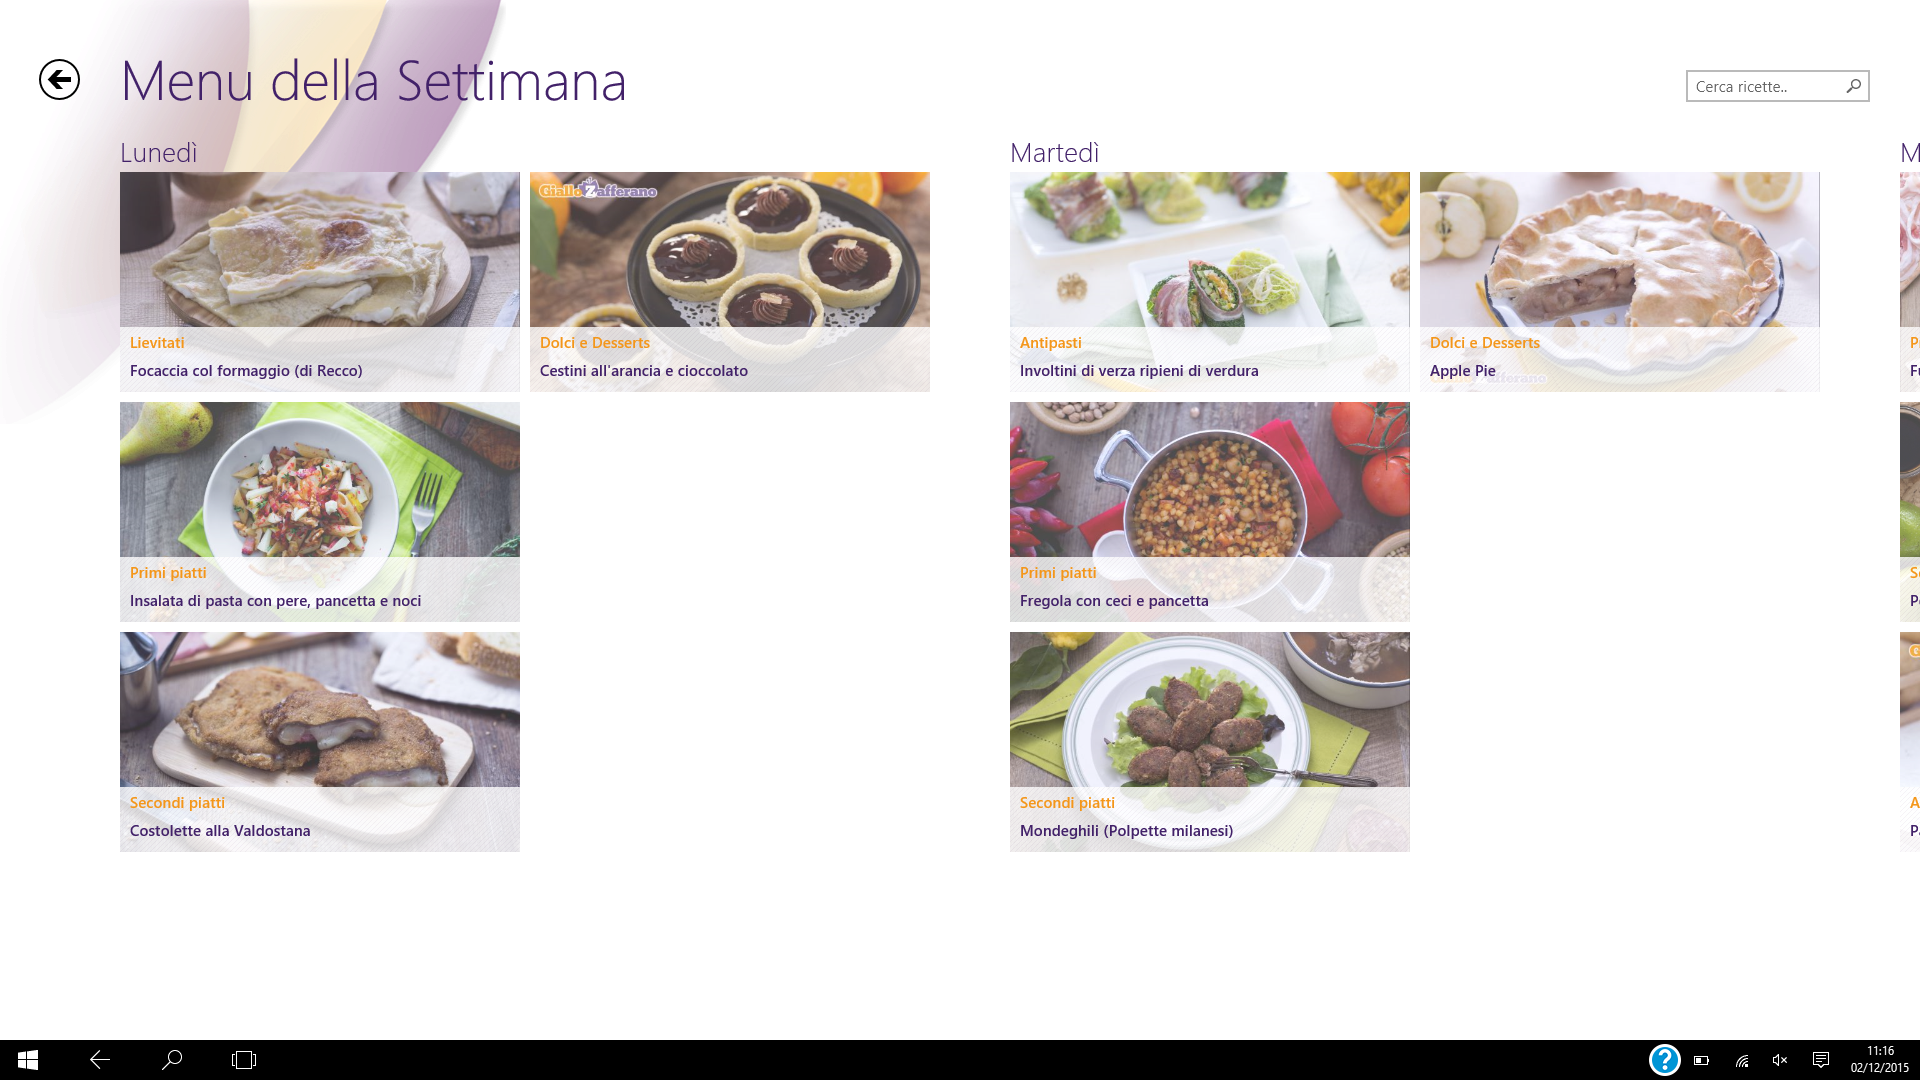
\includegraphics[scale=0.25] {./Giallozafferano/menu_settimana.png}  
\captionof{figure}{Schermata menù della settimana (scroll orizzontale)\\}
\end{center}

\begin{center}
\includegraphics[scale=0.3] {./Giallozafferano/categorie.png}  
\captionof{figure}{Schermata categorie\\}
\end{center}

\begin{center}
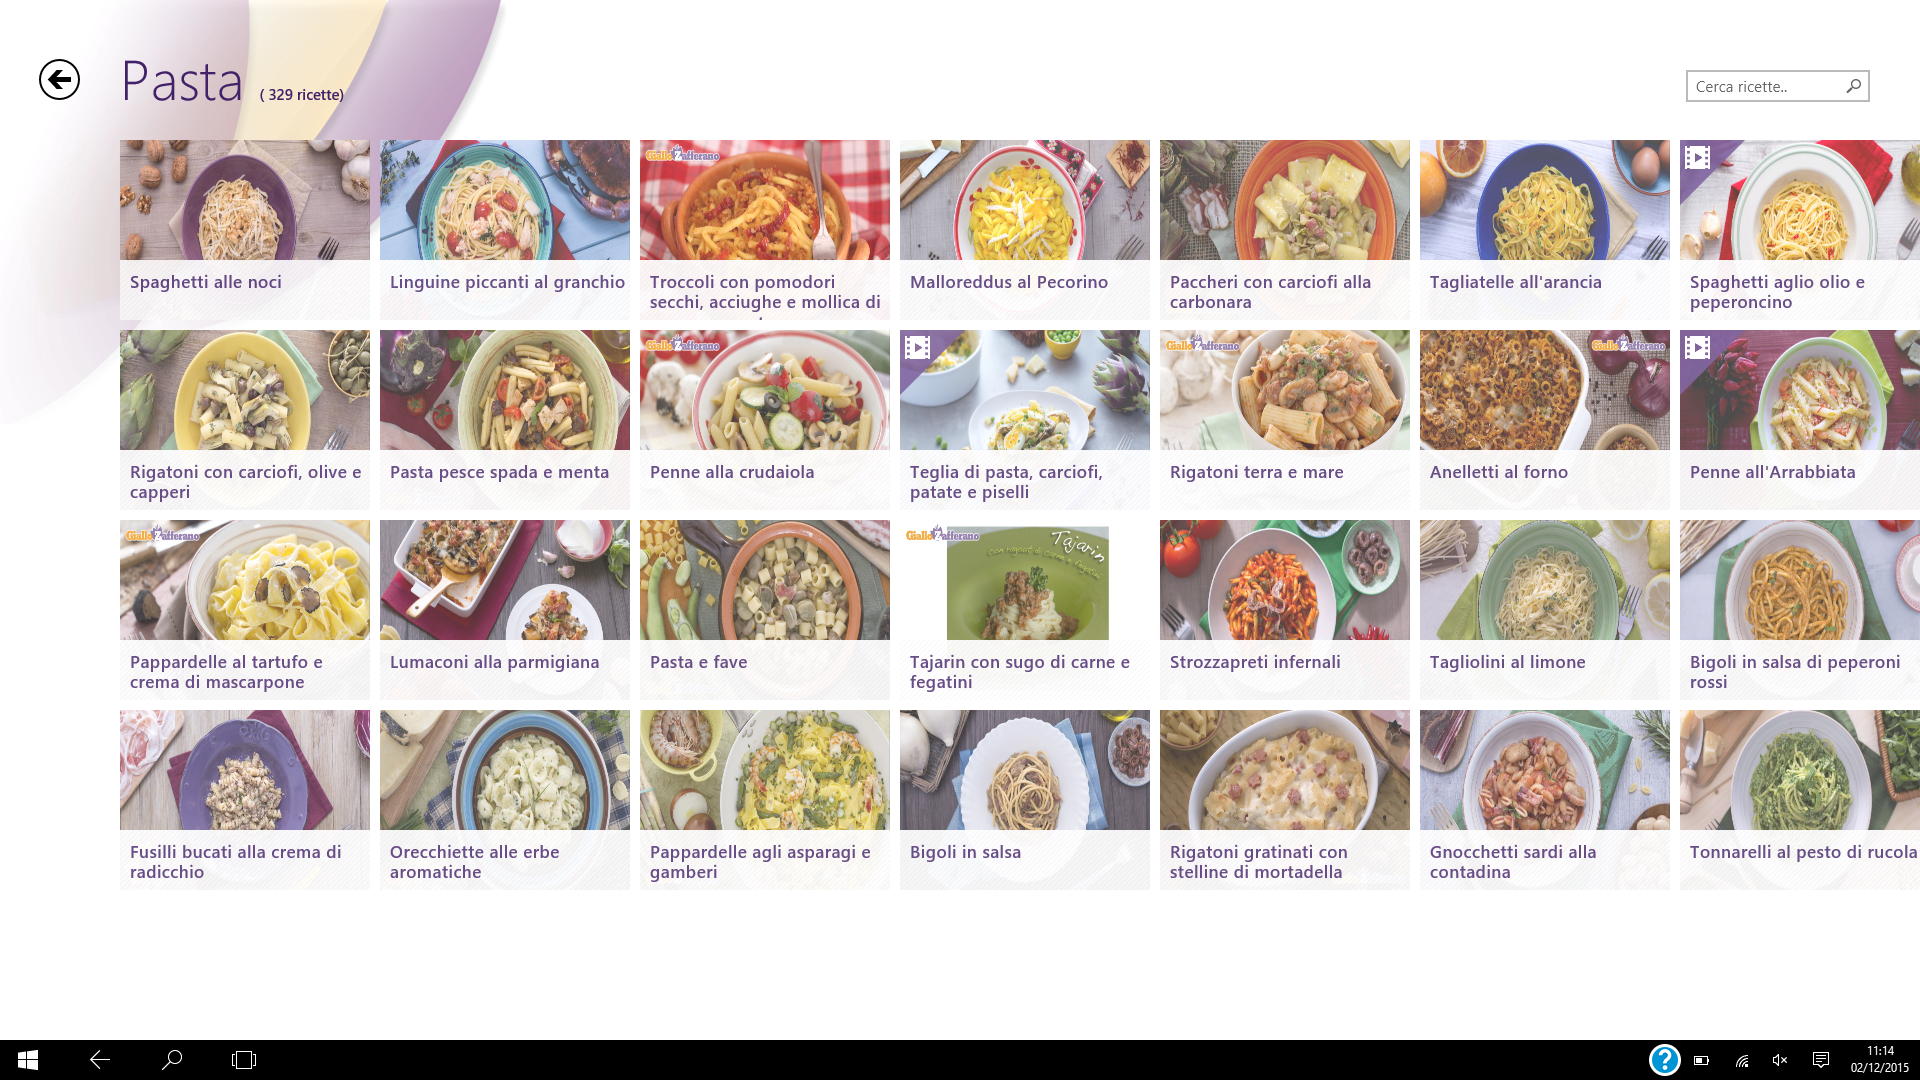
\includegraphics[scale=0.3] {./Giallozafferano/pasta.png}  
\captionof{figure}{Schermata primi piatti : pasta (scroll orizzontale)\\}
\end{center}


L'interfaccia destinata alla presentazione della ricetta risulta ricca di informazioni, con alcuni difetti: nella parte sinistra si propone la videoricetta (se disponibile), insieme alle informazioni base come difficoltà, tempo di cottura e preparazione, ingredienti; scrollando a destra è visionabile la procedure la procedura di preparazione con immagini, conservazione e curiosità.

\begin{center}
\includegraphics[scale=0.275] {./Giallozafferano/ricetta.png}  
\captionof{figure}{Un esempio...\\}
\end{center}

\begin{center}
\includegraphics[scale=0.275] {./Giallozafferano/ricetta_2.png}  
\captionof{figure}{...di ricetta\\}
\end{center}

Anche qui è possibile visualizzare il menù, scrollando dal borso superiore al centro.

\begin{center}
\includegraphics[scale=0.275] {./Giallozafferano/ricetta_menu.png}  
\captionof{figure}{...di ricetta\\}
\end{center}

Il menù superiore non presenta differenze da quello analizzato precedentemente; quello inferiore ha tre funzioni: "\textit{Pin to Start}" per aggiungere la ricetta ai preferiti del sistema operativo, \textit{"Aggiungi ai preferiti"} dell'applicazione e \textit{"Aggiungi alla lista della spesa"}.\\\\
\newpage
Ogni utente ha la possibilità di inserire note personali (private) cliccando sulla matita.

\begin{center}
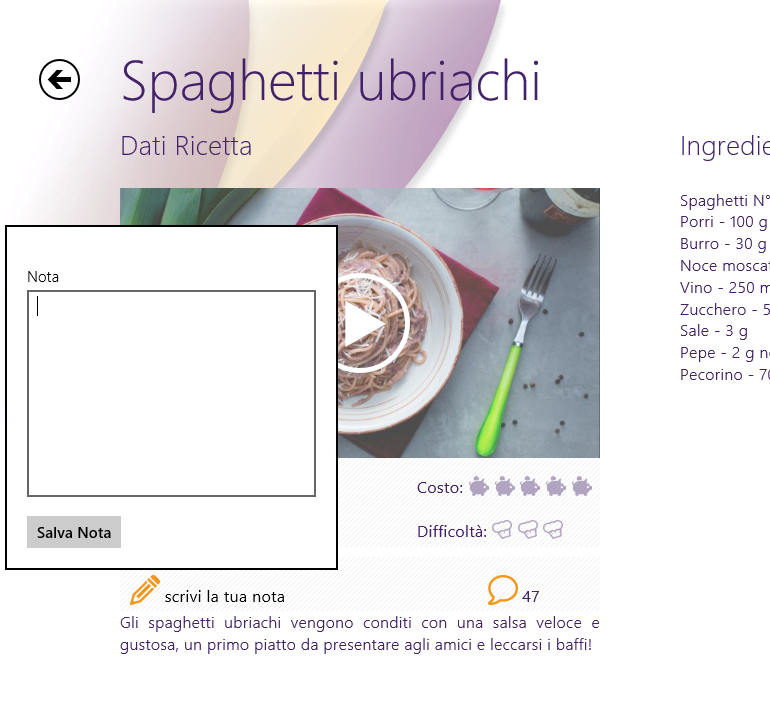
\includegraphics[scale=0.4] {./Giallozafferano/ricetta_nota.png}  
\captionof{figure}{Inserimento di una nota\\}
\end{center}

E' inoltre possibile partecipare ai commenti online per confrontarsi con altri utenti e/o offrire/cercare assistenza.

\begin{center}
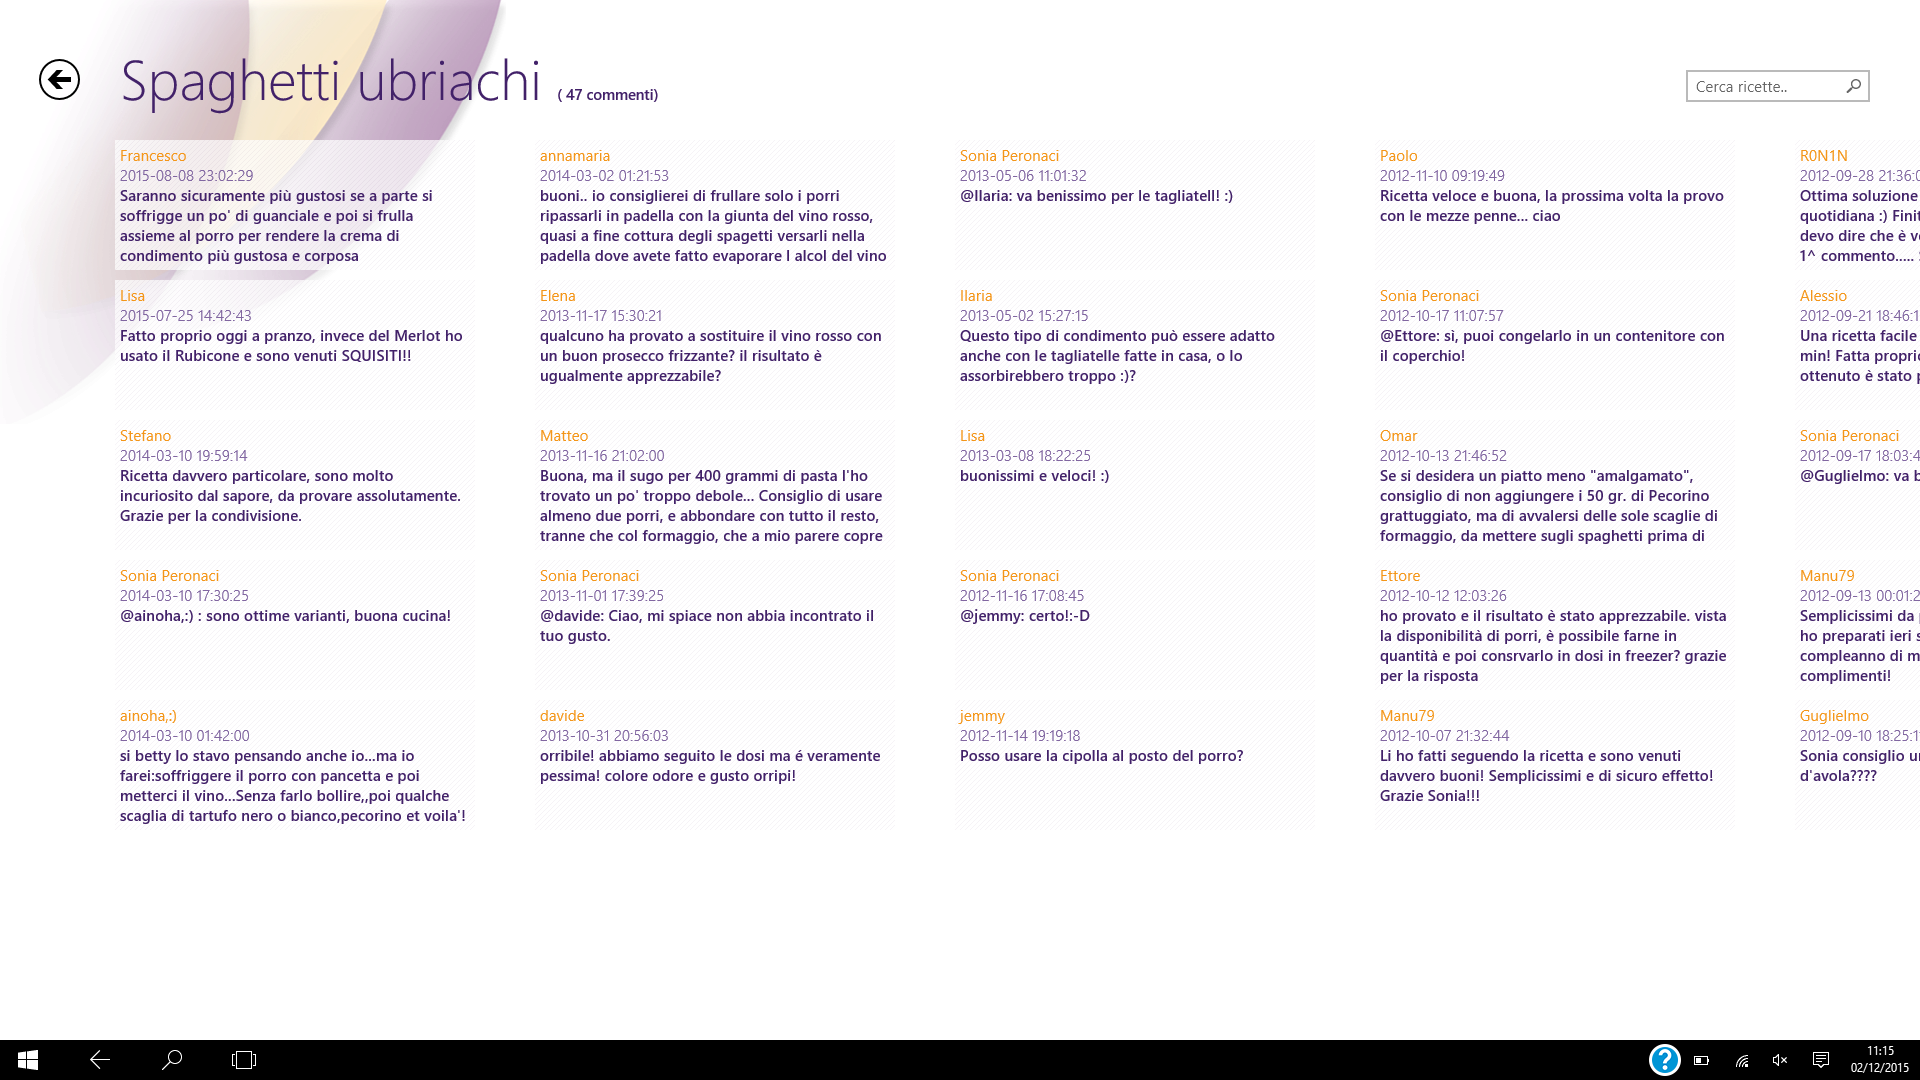
\includegraphics[scale=0.275] {./Giallozafferano/ricetta_commenti.png}  
\captionof{figure}{Schermata commenti\\}
\end{center}

\begin{center}
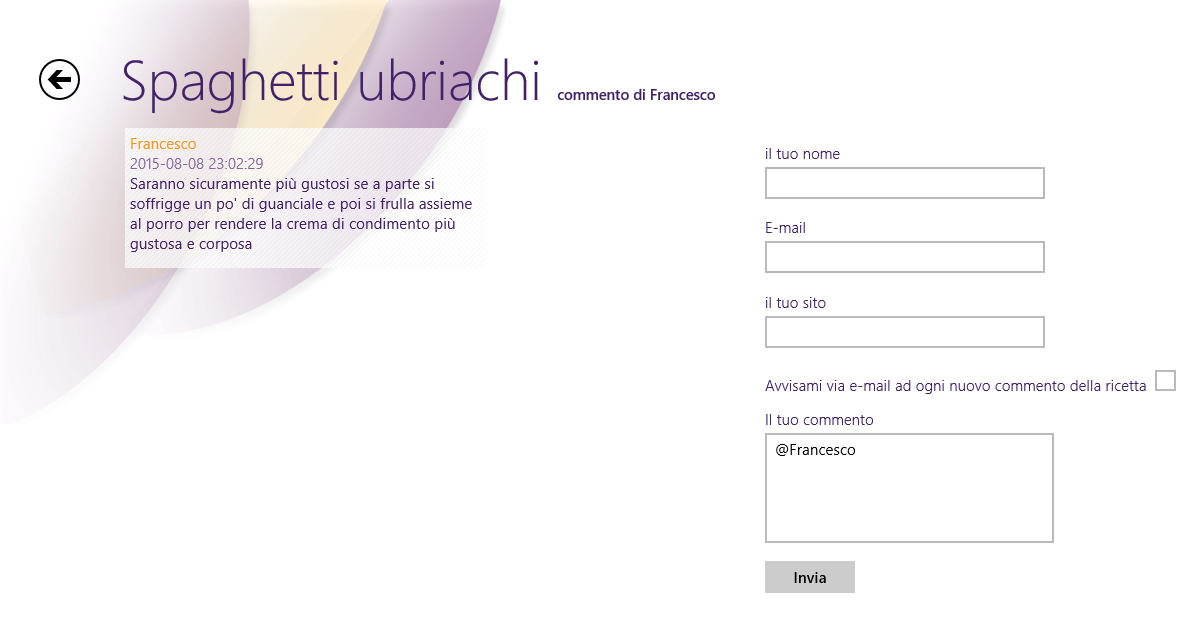
\includegraphics[scale=0.5] {./Giallozafferano/commento_risposta.png}  
\captionof{figure}{Risposta a un commento\\}
\end{center}

Infine la schermata dei preferiti permette facilmente di recuperare ricette salvate precedentemente tra le 3000 proposte.

\begin{center}
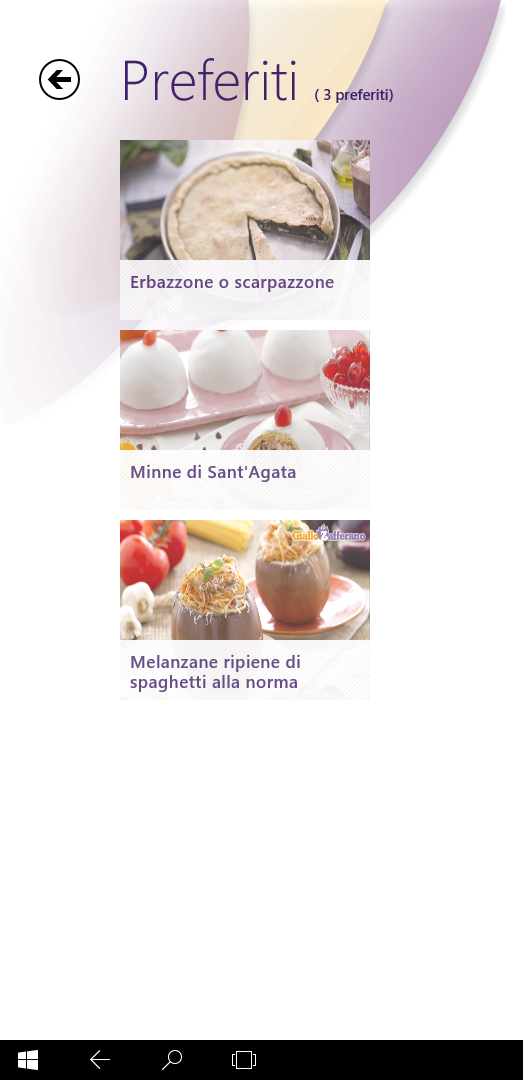
\includegraphics[scale=0.3] {./Giallozafferano/preferiti.png}  
\captionof{figure}{Schermata preferiti\\}
\end{center}

\subsubsection{Allthecooks}
Con oltre 237.000 ricette, Allthecooks è uno dei principale portali culinari internazionali. Ben presente sui social network, offre all'utente un'interfaccia diversa e più funzioni rispetto a GialloZafferano.\\


\begin{center}
\includegraphics[scale=0.275] {./Allthecooks/Home.png}  
\end{center}


\begin{center}
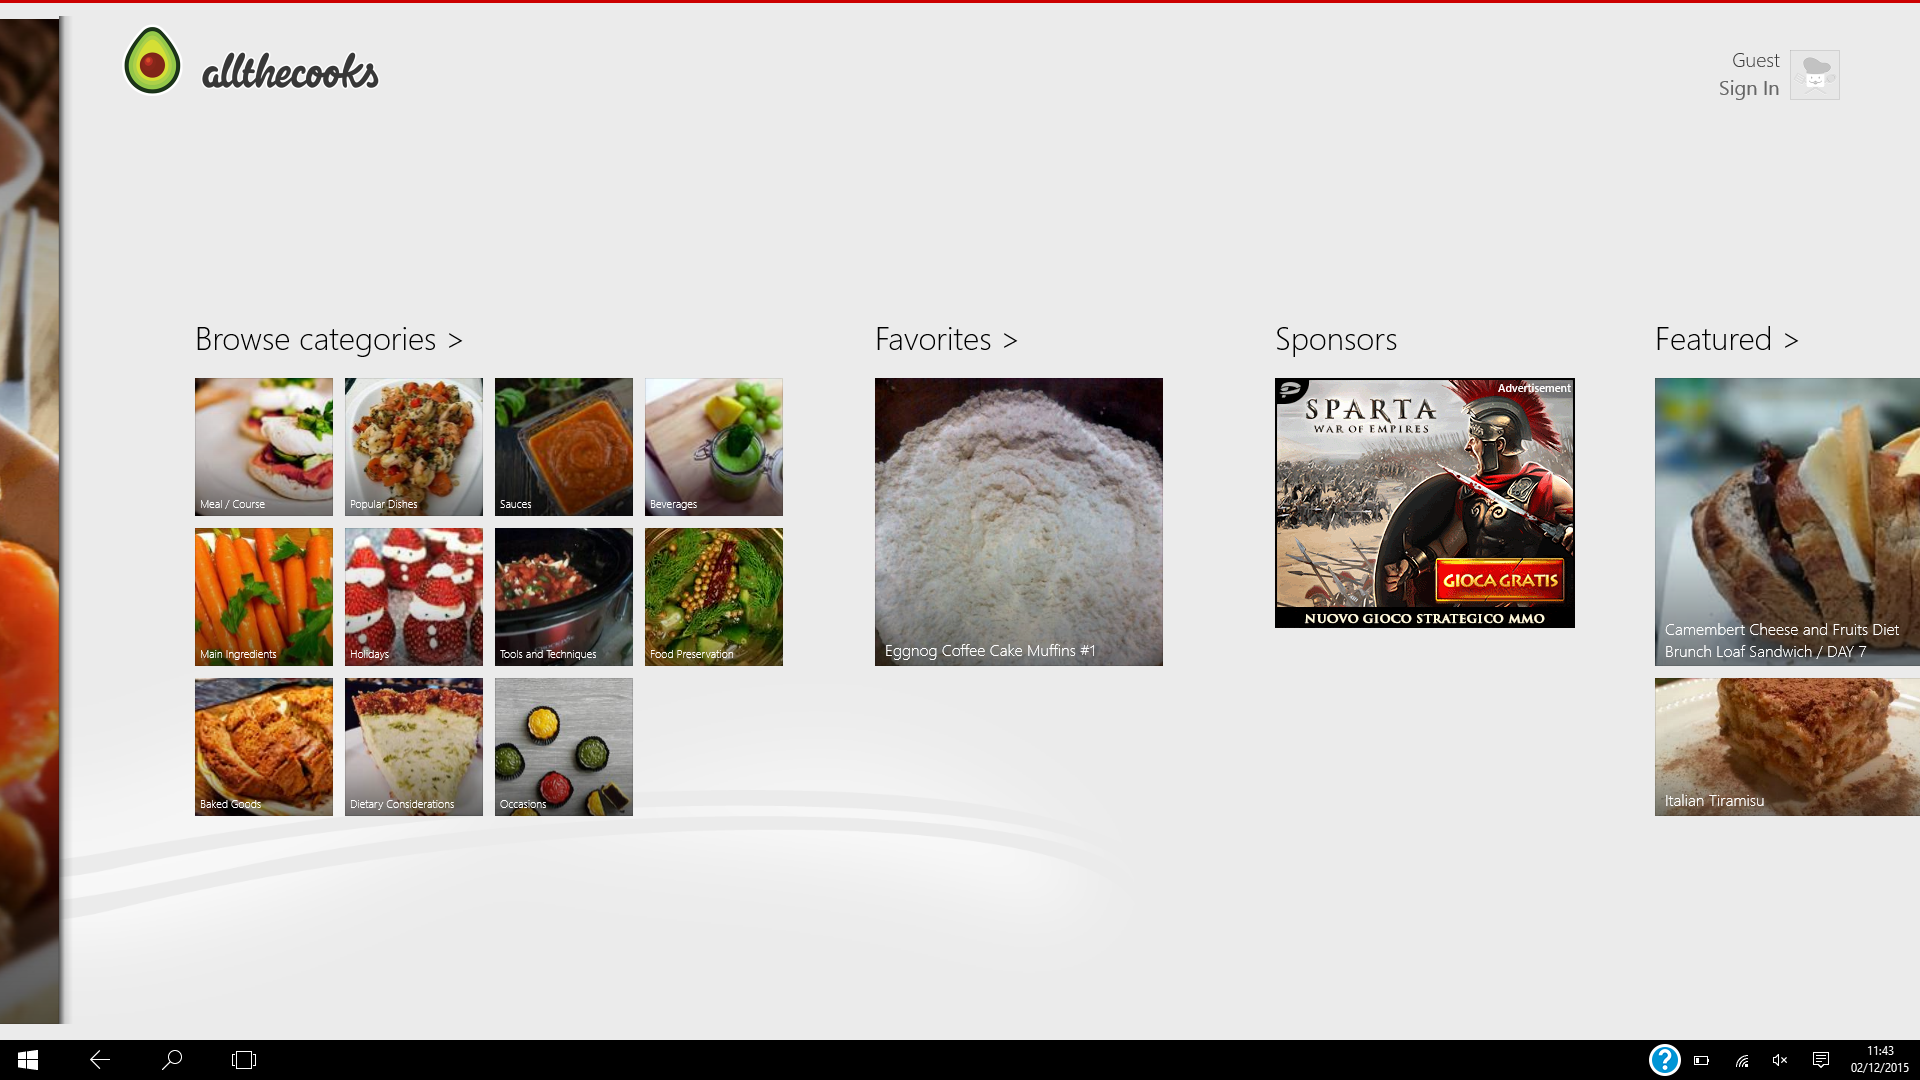
\includegraphics[scale=0.275] {./Allthecooks/home_2.png}  
\captionof{figure}{Schermata principale\\}
\end{center}


\begin{center}
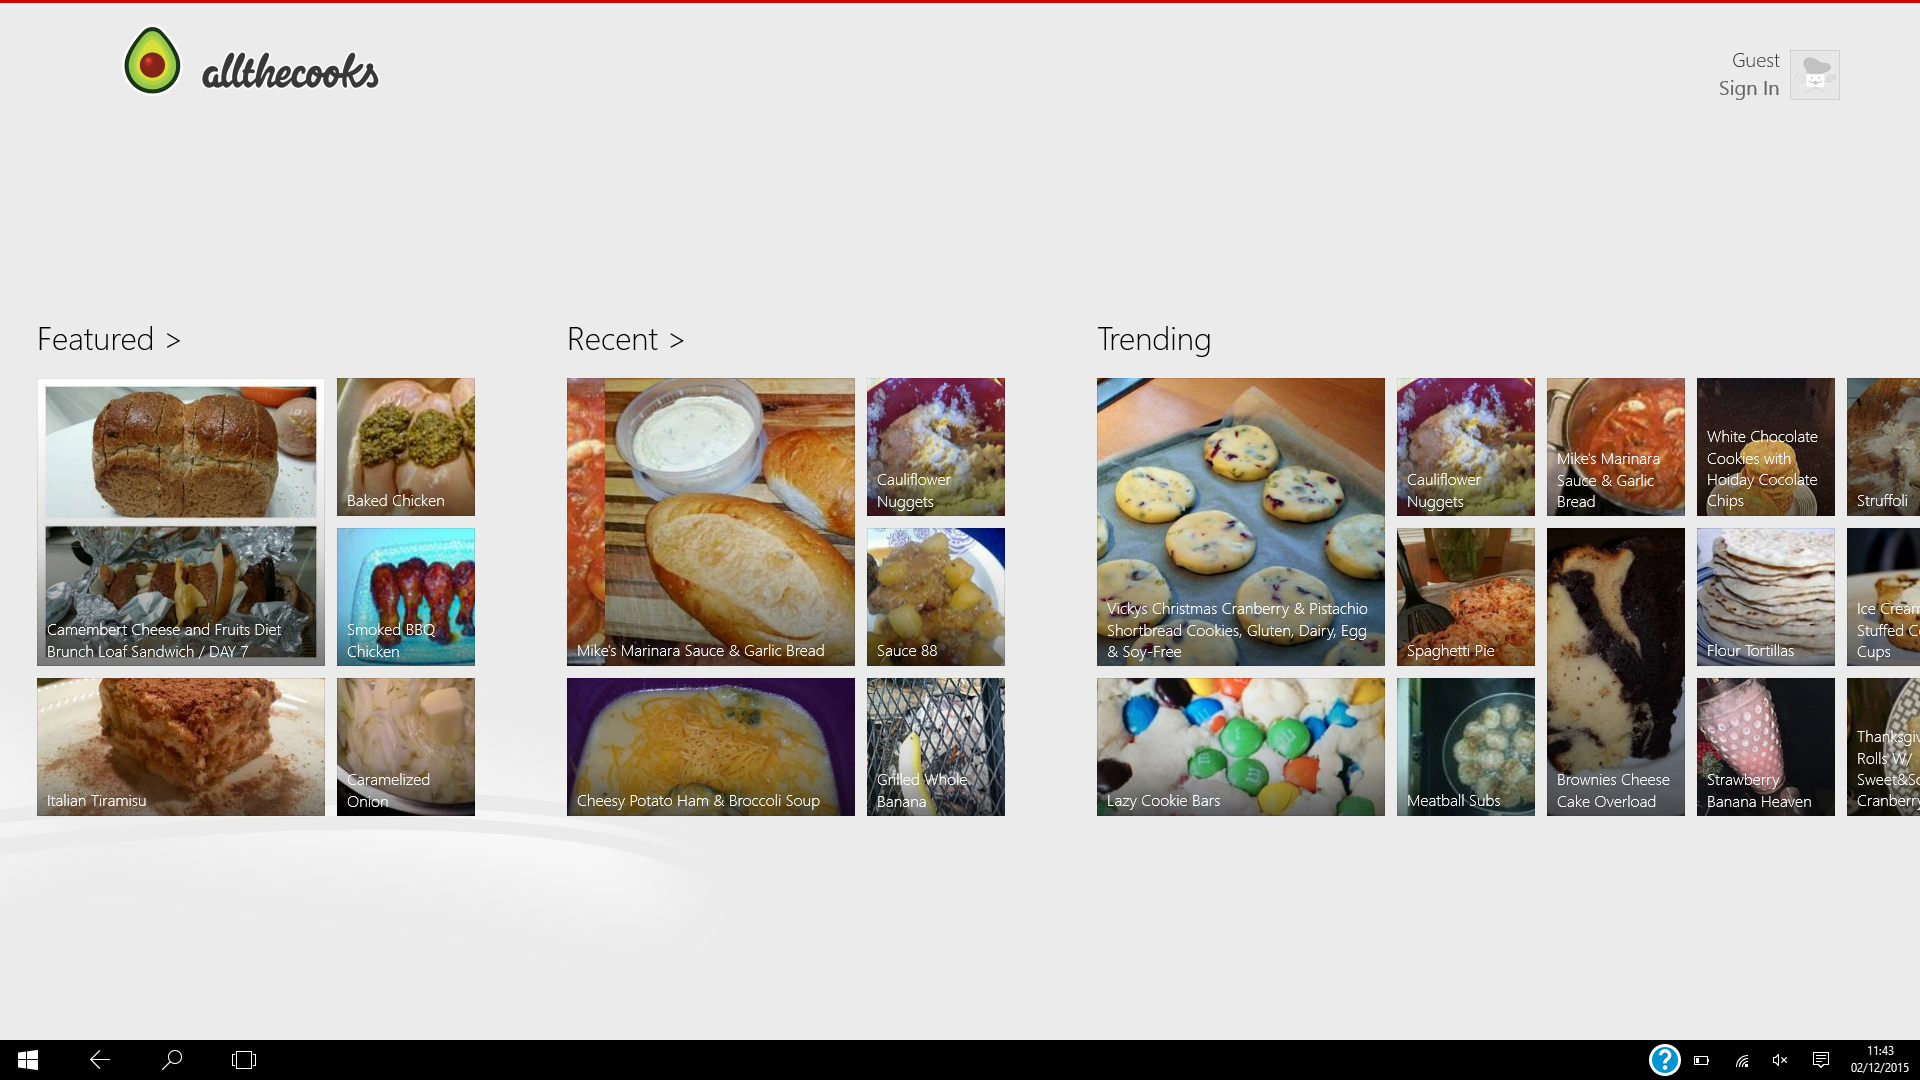
\includegraphics[scale=0.275] {./Allthecooks/home_3.png}  
\captionof{figure}{Schermata principale (scroll orizzontale)\\}
\end{center}

La pagina principale si struttura in orizzontale e prevede un grande slider verticale a sinistra dove vengono visualizzate le ricette più visitate e coerenti con le nostre scelte precedenti.\\
Affianco sono strutturate tutte le sezioni principali come la raccolta delle categorie, le ricette più recenti o quelle più "di moda".\\


\begin{center}
\includegraphics[scale=0.27] {./Allthecooks/categorie.png}  
\captionof{figure}{Schermata categorie (scroll orizzontale)\\}
\end{center}

La schermata principale delle ricette inizialmente mostra tutte le ricette del database, visualizzate a mosaico utilizzando le fotografie caricate dagli autori; inoltre è possibile filtrare i risultati attraverso tag, numero di recensioni/voti e rilevanza.\\


\begin{center}
\includegraphics[scale=0.275] {./Allthecooks/menu.png}  
\captionof{figure}{Schermata categorie con menù\\}
\end{center}

Uno scroll simile a quello già visto per GialloZafferano, visualizza il menù superiore e inferiore insieme.\\
In alto è possibile trovare le funzioni principali legati al profilo (forum, newsletter, notifiche, messaggi e lista della spesa) insieme alla possibilità di tornare alla home o di aggiungere una propria ricetta; in quella inferiore è possibile ricaricare la pagina con un refresh, condividere sui social la pagina in uso o salvare la sezione nei preferiti del sistema operativo.\\


\begin{center}
\includegraphics[scale=0.275] {./Allthecooks/ricetta.png}  
\captionof{figure}{Schermata ricetta (scroll orizzontale)\\}
\end{center}


\begin{center}
\includegraphics[scale=0.275] {./Allthecooks/ricetta_2.png}  
\captionof{figure}{Schermata ricetta (scroll orizzontale)\\}
\end{center}

La schermata distribuisce orizzontalmente tutte le informazioni richieste al momento dell'aggiunta di una ricetta:
\begin{itemize}
\item Un'immagine di copertina, insieme a 5 stelle di voto di apprezzamento
\item Un link al profilo di chi ha aggiunto la ricetta
\item La lista degli ingredienti, automaticamente adattata al numero di porzioni richieste
\item I procedimenti numerati della preparazione
\item Una galleria di fotografie
\item Un'eventuale tabella nutrizionale
\item Una sezione social dove è possibile scegliere dove condividere la ricetta
\end{itemize}

\hspace{-40px}
\begin{minipage}[b]{8.5cm}
	\centering
	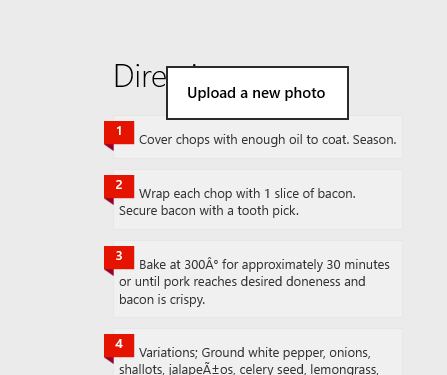
\includegraphics[width=8cm]{./Allthecooks/ricetta_descr_foto.png}
	\captionof{figure}{Add foto al procedimento\\}
\end{minipage}
\ \hspace{2mm}	\hspace{3mm}	\
\begin{minipage}[b]{8.5cm}
	\centering
	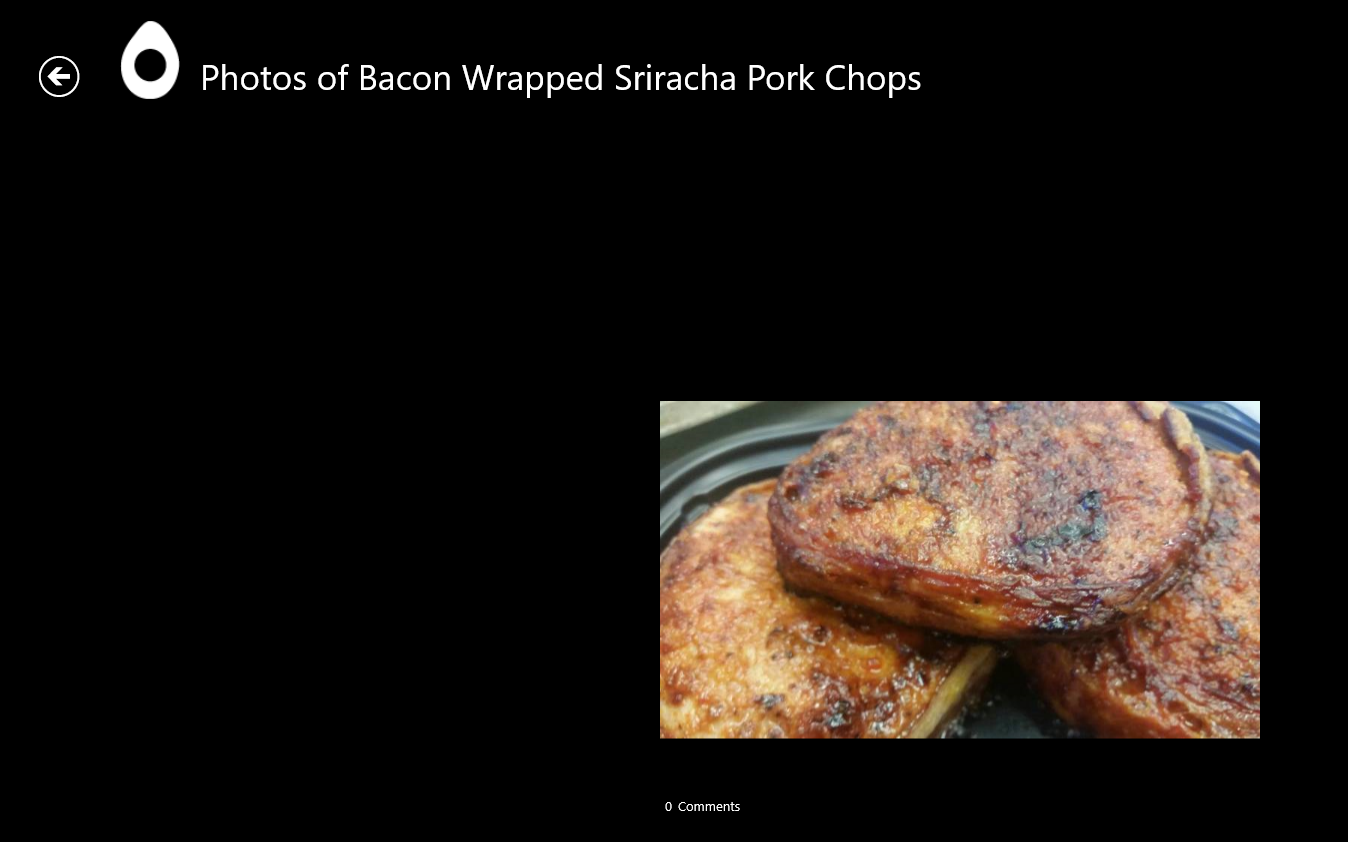
\includegraphics[width=8cm]{./Allthecooks/ricetta_foto.png}
	\captionof{figure}{Schermata galleria ricetta}
\end{minipage}

\begin{center}
\includegraphics[scale=0.27] {./Allthecooks/ricetta_menu.png}  
\captionof{figure}{Schermata ricetta con menù}
\end{center}

Nella schermata ricetta, il menù si arricchisce di nuove funzioni, oltre a quelle già viste:
\begin{itemize}
\item La possibilità di aggiungere la ricetta ai preferiti
\item La possibilità di aggiungere una recensione
\item Si può fare una domanda all'autore
\item Si può aggiungere una fotografia
\item Si possono aggiungere gli ingredienti alla lista della spesa
\item Si può cambiare il sistema metric
\item Si può incrementare la misura del font
\item Stampa della pagina
\end{itemize}


\subsection*{Analisi diretta - Giallozafferano}

\begin{itemize}
\item La schermata principale non occupa interamente lo spazio disponibile e, all'apertura, non vi è un tutorial che ne permetta un veloce apprendimento iniziale. Inoltre non vi è modo di capire che attraverso lo swipe del dito sul margine superiore è possibile visualizzare il menù dell'applicazione.\\ Infine i titoli delle varie sezioni non sono chiaramente cliccabili.

\item Nella pagina di una ricetta, se la difficoltà e/o il tempo di cottura è minimo, la simbologia delle icone non indica adeguatamente il livello, ad esempio 5 salvadanai sbiaditi potrebbero essere confusi con il costo massimo.\\
La lista degli ingredienti è chiaramente visibile, ma non permette di adeguare le porzioni al numero di persone necessarie.\\
Le fotografie non sono ingrandibili, rendendone difficile la visione se il dispositivo in uso è lontano. Non si può condividere la ricetta sui principali social network.\\La sezione delle note è ambigua: non è chiaro se queste note sono personali o pubbliche, vista anche la vicinanza con la sezione dei commenti della community.

\item Non tutte le ricette visualizzano un video esplicativo della preparazione.

\item Non vi è la possibilità di interagire vocalmente con l'applicazione, nè è possibile impostare la grandezza dei testi per facilitare la lettura.

\item Se il menù è visibile, è facile aggiungere gli ingredienti alla lista della spesa. La struttura della pagina "Lista della spesa" è però di difficile uso: è possibile selezionare e spuntare certi ingredienti, ma non è possibile rimuoverli. E' possibile rimuoverli solo attraverso la relativa pagina della ricetta.\\Inoltre se la lista è vuota viene semplicemente visualizzato il titolo senza indicare possibili interazioni o istruzioni.\\
Durante l'uso si sono individuati anche problemi di visualizzazione corretta dei caratteri.

\begin{center}
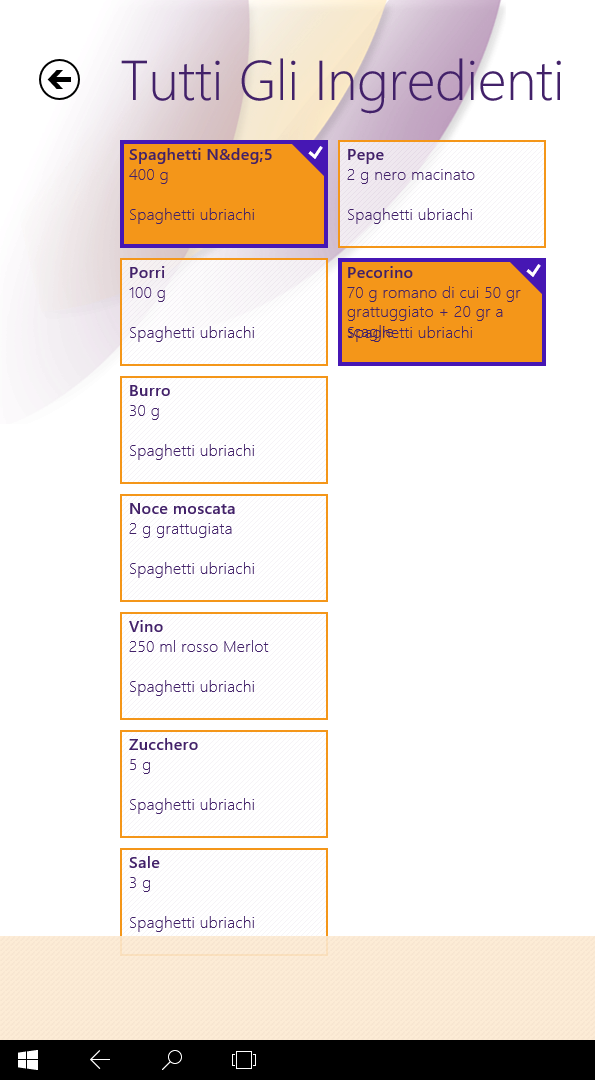
\includegraphics[scale=0.27] {./Giallozafferano/lista_spesa_selezione_1.png}  
\captionof{figure}{Bug visualizzazione caratteri}
\end{center}
\end{itemize}

\subsection*{Analisi diretta - AlltheCooks}

\begin{itemize}
\item La schermata principale occupa interamente lo spazio disponibile ma, all'apertura, non vi è un tutorial che ne permetta un veloce apprendimento iniziale. Inoltre non vi è modo di capire che attraverso lo swipe del dito sul margine superiore è possibile visualizzare il menù dell'applicazione.\\La sezione "panoramica" di sinistra ha lo scroll verticale, ma ci si aspetta di aprire la ricetta cliccando sulla foto, anzichè sul tasto "Learn".\\Non è chiaro che la homepage ha lo scroll orizzontale.

\item Nella pagina di una ricetta, non vi è traccia di indicazioni sul tempo di cottura e difficoltà di preparazione.\\
Vengono mostrate 5 stelle per mostrare il voto alla ricetta, ma non è chiaro come dare un proprio voto.\\
Cliccando su un'istruzione, compare un pop-up per l'inserimento di una fotografia, ma non è chiaro se chiunque può o solo l'autore.\\

\item La barra di ricerca permette l'inserimento di termini, ma l'ok è possibile solo tramite il tasto inivio e non mediante il click sulla lente.

\item Nella ricerca delle ricette, se vengono filtrate per categoria, spesso sono ripetute più volte nei risultati.\\Inoltre è lecito inserire ricette senza fotografie di supporto.

\item L'animazione di caricamento pagina è visualizzata in alto a destra e non è subito visibile e chiara.

\item Quando si aggiunge degli ingredienti alla lista della spesa, non vi è la possibilità di aggiungerli tutti se non selezionandone uno a uno; inoltre nell'apposita pagina non è più presente a quale ricetta facevano riferimento.

\item Nella sezione Forum, il pulsante per inserire una nuova discussione non è di chiara comprensione.

\item L'applicazione permette l'azione "Pin to Start", ma solo cliccandola è chiaro che si riferisce allo Start del sistema operativo.

\end{itemize}

\subsection*{Analisi inversa - Giallozafferano}

A partire dalle 10 euristiche di Nielsen e Molich, individuiamo quali linee guida sono state violate:

\begin{itemize}
\item La linea guida 1 è sicuramente violata dall'errata posizione dell'animazione di loading, poco chiara e poso centrata; inoltre se si accede a una ricetta, l'utente non è informato sul percorso fatto per arrivarci.\\La preparazione della ricetta è più guidata dai numeri sulle immagini che non dal testo che le accompagna.

\item La linea guida 2 è violata nel momento in cui la ricetta è scritta da professionisti: capita spesso che nelle fasi di preparazioni vengano utilizzati termini non adatti a tutti gli utenti. L'applicazione non offre una diversa terminologia a secondo del livello di esperienza impostato dall'utente.

\item Linea guida 3: l'unica interazione possibile dell'utente è nella compilazione di domande/risposte con la community. In questo caso però, nel momento in cui si compila il campo di testo e si torna indietro con l'apposito pulsante, si perderà tutto il contenuto scritto e sarà necessario reinserirlo nuovamente.

\item La linea guida 4 è violata nell'interazione con la community: quando si invia un commento, il sistema non chiede conferma all'utente.

\item La linea guida 5  è violata, data l'assenza di messaggi di errore di qualsiasi tipo. Ad esempio se si tenta di inserire un commento vuoto, il pulsante Invia non notifica nulla.

\item La linea 6 è pesantemente violata dall'assenza di un riferimento al menù, visibile solo mediante lo swipe del margine superiore dello schermo. Non vi è mai una sezione help disponibile.

\item Come già detto nella linea guida 5, l'applicazione non offre nessun tipo di messaggio d'errore. La linea guida 9 è violata.

\item L'applicazione non offre nessun tipo di documentazione o tutorial. La linea guida 10 è violata.
\end{itemize}

\subsection*{Analisi inversa - AlltheCooks}

\begin{itemize}
\item La linea guida 1 è sicuramente violata dall'errata posizione dell'animazione di loading, poco chiara e posizionata in alto a destra; inoltre se si accede a una ricetta, l'utente non è informato sul percorso fatto per arrivarci.\\

\item La linea guida 2 è violata nel momento in cui la ricetta è scritta troppo informalmente: la libertà di inserimento data dall'applicazione non prevede un controllo preliminare dei contenuti aggiunti, quindi il linguaggio familiare si scontra spesso con istruzioni incomplete, a volte addirittura assenti.

\item Linea guida 3: nell'inserimento delle ricette, non è presente una funzione di "redo" una volta abbandonata la finestra. Inoltre se si ricarica la finestra, non viene mostrato il popup di conferma, come viene fatto se si tenta di tornare indietro.

\item La linea guida 4 è violata nell'inserimento delle ricette; ad esempio non vi è una chiara distinzione tra "ingredient" o "ingredient group".

\item La linea guida 5  è violata nell'inserimento delle ricette: ogni errore commesso durante l'input, viene mostrato solo nel riquadro finale e non segnalando il form stesso.

\item La linea 6 è pesantemente violata dall'assenza di un riferimento al menù, visibile solo mediante lo swipe del margine superiore dello schermo. Non vi è mai una sezione help disponibile.

\item La homepage raggruppa molte sezioni, rendendo la grafica confusa e poco minimale. Inoltre la sezione categorie dipende dalle sezioni di filtro, piuttosto che da categorie preimpostate. E' violata la linea guida 8.

\item L'applicazione non offre nessun tipo di documentazione o tutorial. La linea guida 10 è violata.
\end{itemize}






\end{document}